\documentclass{article}
\usepackage[utf8x]{inputenc}
\usepackage{ucs}
\usepackage{amsmath} 
\usepackage{amsfonts}
\usepackage{marvosym}
\usepackage{wasysym}
\usepackage{upgreek}
\usepackage[english,russian]{babel}
\usepackage{graphicx}
\usepackage{float}
\usepackage{textcomp}
\usepackage{hyperref}
\usepackage{geometry}
  \geometry{left=2cm}
  \geometry{right=1.5cm}
  \geometry{top=1cm}
  \geometry{bottom=2cm}
\usepackage{tikz}
\usepackage{ccaption}
\usepackage{multicol}
\usepackage{subfigure}

\hypersetup{
   colorlinks=true,
   citecolor=blue,
   linkcolor=black,
   urlcolor=blue
}

\usepackage{listings}
\usepackage{textcomp}
%\setlength{\columnsep}{1.5cm}
%\setlength{\columnseprule}{0.2pt}

\usepackage[absolute]{textpos}

\usepackage{colortbl,graphicx,tikz}
\definecolor{X}{rgb}{.5,.5,.5}


\begin{document}
\pagenumbering{gobble}

\lstdefinestyle{myCustomCStyle}{
  language=C,
  basicstyle=\linespread{1.1}\ttfamily,
  columns=fixed,
  fontadjust=true,
  basewidth=0.5em,
  keywordstyle=\color{blue}\bfseries,
  commentstyle=\color{gray},
  stringstyle=\ttfamily\color{orange!50!black},
  showstringspaces=false,
  numbersep=5pt,
  numberstyle=\tiny\color{black},
  numberfirstline=true,
  stepnumber=1,   
  numbersep=10pt,
  backgroundcolor=\color{white},
  showstringspaces=false,
  captionpos=b,
  breaklines=true,
  breakatwhitespace=true,
  xleftmargin=.2in,
  extendedchars=\true,
  keepspaces = true,
  upquote = true,
  emph = {size_t},
  emphstyle={\color{blue}\bfseries},
}


\lstdefinestyle{heapExamplesStyle}{
  style=myCustomCStyle,
  framexleftmargin=5mm, 
  frame=shadowbox, 
  rulesepcolor=\color{gray}
}

\lstset{style=myCustomCStyle}
\lstset{literate=%
   *{0}{{{\color{red!20!violet}0}}}1
    {1}{{{\color{red!20!violet}1}}}1
    {2}{{{\color{red!20!violet}2}}}1
    {3}{{{\color{red!20!violet}3}}}1
    {4}{{{\color{red!20!violet}4}}}1
    {5}{{{\color{red!20!violet}5}}}1
    {6}{{{\color{red!20!violet}6}}}1
    {7}{{{\color{red!20!violet}7}}}1
    {8}{{{\color{red!20!violet}8}}}1
    {9}{{{\color{red!20!violet}9}}}1
}
\newpage

\title{Семинар \#5: Сегменты памяти.\vspace{-5ex}}\date{}\maketitle
\section*{Обзор основных сегментов памяти}
\begin{multicols}{2}
\begin{center}
\includegraphics[scale=1.1]{../images/memory_layout.png}
\end{center}
\columnbreak
\begin{enumerate}
\item \textbf{Сегмент памяти Стек (Stack)} \\
\begin{itemize}
\item При обычном объявлении переменных (в том числе массивов) внутри функций все они создаются в стеке: 
\begin{lstlisting}
int a; 
int array[10];
\end{lstlisting}


\item Память на локальные переменные функции выделяется при вызове этой функции и освобождается при завершении функции.
\item Маленький размер (несколько мегабайт, зависит от настроек операционной системы).
\item Выделение памяти происходит быстрее чем в куче.
\end{itemize}
\item \textbf{Сегмент памяти Куча (Heap)} \\
\begin{itemize}
\item Выделеть память в куче можно с помощью стандартной функции \texttt{malloc}: \\
\begin{lstlisting}
int* p = malloc(10 * sizeof(int));
\end{lstlisting}
\item Освободить память в куче можно с помощью стандартной функции \texttt{free}:
\begin{lstlisting}
free(p);
\end{lstlisting}
\item Можно выделить намного больше памяти, чем в стеке.
Как правило, можно использовать всю свободную память системы.
\item Выделение памяти происходит медленней чем в стеке.
\end{itemize}
\end{enumerate}
\end{multicols}

\begin{enumerate}
\setcounter{enumi}{2}

\item \textbf{Сегмент памяти Данные (Data)}
\begin{itemize}
\item В этом сегменте хранятся глобальные и статические переменные а также строковые литералы.
\item Можно выделить намного больше памяти, чем в стеке.
Как правило, можно использовать всю свободную память системы.
\item Выделение памяти происходит при запуске программы, а освобождение при завершении программы.
\end{itemize}

\item \textbf{Сегмент памяти Текст (Text)}
\begin{itemize}
\item В этом сегменте хранится машинный код программы (Код на языке C, сначала, переводится в код на языке Ассемблера, а потом в машинный код.).
\item Адрес функции - адрес первого байта инструкций в этом сегменте.
\end{itemize}
\end{enumerate}


\newpage
\section*{Сегмент памяти Куча}
Основные функции для динамического выделения памяти в куче содержатся в библиотеке \texttt{stdlib.h}:
\begin{itemize}
\item \texttt{void* malloc(\textbf{size\_t} n)} -- выделяет \texttt{n} байт в сегменте памяти Куча и возвращает указатель типа \texttt{void*} на начало этой памяти. Если память выделить не получилось (например памяти не хватает), то функция вернёт значение \texttt{NULL}. \\
\item \texttt{void free(\textbf{void*} p)} -- освобождает выделенную память. Если ненужную память вовремя не освободить, то она останется помеченной, как занятая до момента завершения программы. Произойдёт так называемая утечка памяти. Правило при работе с \texttt{free}: число вызовов \texttt{free} должно быть равно числу вызовов \texttt{malloc}.\\
\item \texttt{void* realloc(\textbf{void*} p, \textbf{size\_t} new\_n)} -- перевыделяет выделенную память. Указатель \texttt{p} должен указывать на ранее выделенную память. Память, на которую ранее указывал \texttt{p}, освободится. \\
Если память перевыделить не получилось (например памяти не хватает), то функция вернёт значение \texttt{NULL}. При этом указатель \texttt{p} будет продолжать указывать на старую память, она не освободится.\\
\end{itemize}

Давайте рассмотрим как работать с этими функциями. Предположим, что мы хотим создать в куче одну переменную типа \texttt{int}. Так как мы знаем, что \texttt{int} занимает 4 байта, то мы можем написать следующее:
\begin{lstlisting}
int* p = (int*)malloc(4);
\end{lstlisting}
Обратите внимание на то что мы привели указатель \texttt{void*}, который возвращает \texttt{malloc}, к указателю \texttt{int*}.\\
В языке \texttt{C} такое приведение можно не писать, а в языке \texttt{C++} это обязательно. Однако, такое использование \texttt{malloc} не совсем верно, так как тип \texttt{int} не всегда имеет размер 4 байта. На старых системах он может иметь размер 2 байта, а на очень новых -- даже 8 байт. Поэтому лучше использовать оператор \texttt{sizeof}.\\

Схематически выделение одного \texttt{int}-а в куче можно изобразить следующим образом:
 
 
\noindent\begin{minipage}{.50\textwidth}
\begin{lstlisting}
#include <stdio.h>
#include <stdlib.h>
int main()
{
    int* p = (int*)malloc(sizeof(int));
    *p = 123;
    printf("%i\n", *p);
    free(p);
}
\end{lstlisting}
\end{minipage}\hfill
\begin{minipage}{.40\textwidth}
\includegraphics[scale=0.7]{../images/malloc_class_tasks/heap_int.png}
\end{minipage} 

Конечно, основное преемущество кучи это её размер, который ограничен только доступной физической памятью. Поэтому на куче обычно выделяют не одиночные переменные, а массивы. Вот схематическое изображение выделения массива из 4-х элементов на куче:\\
\noindent\begin{minipage}{.50\textwidth}
\begin{lstlisting}
#include <stdio.h>
#include <stdlib.h>
int main()
{
    int* p = (int*)malloc(4 * sizeof(int));
    p[0] = 11;
    p[1] = 22;
    p[2] = 33;
    p[3] = 44;
    printf("%i\n", p[2]);
    free(p);
}
\end{lstlisting}
\end{minipage}
\begin{minipage}{.40\textwidth}
\includegraphics[scale=0.68]{../images/malloc_class_tasks/heap_int_array.png}
\end{minipage}

Благодаря тому, что к указателям можно применять квадратные скобки, работа с указателем \texttt{p} ничем не отличается от работы с массивом размером в 4 элемента.\\


\subsection*{Обработка ошибок при выделении памяти}
Если при вызове \texttt{malloc} произошла какая-либо ошибка, например, вы просите больше памяти, чем осталось, то \texttt{malloc} вернёт нулевой указатель равный \texttt{NULL} (\texttt{NULL} -- это просто константа, равная нулю). Поэтому при каждом вызове \texttt{malloc} желательно проверять, сработал ли он корректно:
\begin{lstlisting}
int* p = (int*)malloc(1000 * sizeof(int));
if (p == NULL) 
{
    printf("Error! Out of memory.\n");
    exit(1);
}
\end{lstlisting}
В учебных примерах мы это делать не будем, чтобы код оставался коротким и более понятным, однако при разработке на языках C и C++ крайне важно делать эту проверку.

\subsection*{Утечки памяти}
Если вы забудете освободить память с помощью \texttt{free}, когда она перестанет быть нужна, то программа будет использовать больше памяти чем нужно. Произойдёт так называемая утечка памяти. Если в программе есть утечки памяти, то с течением времени она будет потреблять всё больше и больше памяти. Но при завершении программы вся память, конечно, освобождается.
\begin{lstlisting}
#include <stdlib.h>
void func(int n) 
{
    int* p = (int*)malloc(n * sizeof(int));
    // ... забыли вызвать free
}
int main() 
{
    func(10000);
    // После выполнения функции func мы не сможем освободить память, даже если захотим
    // так как не знаем указатель на начало этой памяти
    
    // При каждом вызове функции будет тратиться память
    for (int i = 0; i < 100; ++i)
        func(10000);
}
\end{lstlisting}
Существуют специальные программы, которые проверяют нет ли у вас в программе утечек памяти. Одна из таких программ -- \texttt{valgrind} на ОС семейства \texttt{Linux}. Чтобы её использовать, нужно просто написать в терминале:
\begin{verbatim}
valgrind ./a.out
\end{verbatim}


\subsection*{Повторное освобождение той же памяти}
Если вы попробуете освободить уже освобождённый участок памяти, это приведёт к неопределённому поведению:
\begin{lstlisting}
int* p = (int*)malloc(1000 * sizeof(int));
free(p);
// ...
free(p); // Забыли, что p уже освободили и освобождаем снова, это UB
\end{lstlisting}
Для минимизации шанса возникновения этой ошибки, можно занулять указатель после освобождения памяти:
\begin{lstlisting}
int* p = (int*)malloc(1000 * sizeof(int));
free(p);
p = NULL;
// ...
free(p); // Функция free ничего не будет делать, если ей передать NULL. Тут нет ошибки.
\end{lstlisting}


\section*{Примеры создания объектов в куче}

Напишем код, который будет создавать в куче различные объекты. В каждом примере напечатаем созданные в куче объекты и освободим всю память, которую вы выделили. Исходный код всех примеров из этого раздела можно найти в папке \texttt{examples}.
\begin{enumerate}


\item Один символ:\\
\noindent\begin{minipage}{.50\textwidth}
\begin{lstlisting}[style=heapExamplesStyle]
char* p = (char*)malloc(sizeof(char));
*p = 'A';

printf("%c\n", *p);
free(p);
\end{lstlisting}
\end{minipage}\hfill
\begin{minipage}{.40\textwidth}
\includegraphics[scale=0.7]{../images/malloc_class_tasks/heap_char.png}
\end{minipage}
\quad\\
\quad\\


\item Массив из трёх элементов типа \texttt{float}:\\
\noindent\begin{minipage}{.50\textwidth}
\begin{lstlisting}[style=heapExamplesStyle]
float* p = (float*)malloc(sizeof(float) * 3);
p[0] = 1.1;
p[1] = 2.2;
p[2] = 3.3;

for (size_t i = 0; i < 3; ++i)
    printf("%f ", p[i]);
printf("\n");
free(p);
\end{lstlisting}
\end{minipage}\hfill
\begin{minipage}{.4\textwidth}
\includegraphics[scale=0.7]{../images/malloc_class_tasks/heap_double_array.png}
\end{minipage}
\quad\\
\quad\\


\item Строку (массив \texttt{char}) \texttt{"Cats and Dogs"}:\\
\noindent\begin{minipage}{.50\textwidth}
\begin{lstlisting}[style=heapExamplesStyle]
char* p = (char*)malloc(sizeof(char) * 14);
strcpy(p, "Cats and Dogs");

printf("%s\n", p);
free(p);
\end{lstlisting}
\end{minipage}\hfill
\begin{minipage}{.40\textwidth}
\includegraphics[scale=0.7]{../images/malloc_class_tasks/heap_char_array.png}
\end{minipage}
\quad\\
\quad\\


\item Структуру \texttt{Book} из семинара на структуры:\\
\noindent\begin{minipage}{.50\textwidth}
\begin{lstlisting}[style=heapExamplesStyle]
Book* p = (Book*)malloc(sizeof(Book));
strcpy(p->title, "War and Peace");
p->pages = 1225;
p->price = 2000.0;

printf("Book: %s, Pages: %i, Price: %f\n", pb->title, pb->pages, pb->price);

free(p);
\end{lstlisting}
\end{minipage}\hfill
\begin{minipage}{.40\textwidth}
\includegraphics[scale=0.7]{../images/malloc_class_tasks/heap_struct_book.png}
\end{minipage}
\quad\\
\quad\\


\newpage
\item Указатель, который указывает на число \texttt{int}:\\
\noindent\begin{minipage}{.50\textwidth}
\begin{lstlisting}[style=heapExamplesStyle]
int** p = (int**)malloc(sizeof(int*));

*p = (int*)malloc(sizeof(int));

**p = 123;

printf("%i\n", **p);
free(*p);
free(p);
\end{lstlisting}
\end{minipage}\hfill
\begin{minipage}{.40\textwidth}
\includegraphics[scale=0.7]{../images/malloc_class_tasks/heap_pointer_int.png}
\end{minipage}
\quad\\
\quad\\

\item Указатель, который указывает на число \texttt{int}, которое находится в стеке:\\
\noindent\begin{minipage}{.50\textwidth}
\begin{lstlisting}[style=heapExamplesStyle]
int a = 123;

int** p = (int**)malloc(sizeof(int*));
*p = &a;

printf("%i\n", **p);
free(p);
\end{lstlisting}
\end{minipage}\hfill
\begin{minipage}{.40\textwidth}
\includegraphics[scale=0.7]{../images/malloc_class_tasks/heap_pointer_int_stack.png}
\end{minipage}
\quad\\
\quad\\


\item Массив из указателей на \texttt{int}:\\
\noindent\begin{minipage}{.50\textwidth}
\begin{lstlisting}[style=heapExamplesStyle]
int** p = (int**)malloc(3 * sizeof(int*));

for (size_t i = 0; i < 3; ++i)
    p[i] = (int*)malloc(sizeof(int));

*p[0] = 100;
*p[1] = 200;
*p[2] = 300;

for (size_t i = 0; i < 3; ++i)
    printf("%i ", *p[i]);
printf("\n");

for (size_t i = 0; i < 3; ++i)
    free(p[i]);
free(p);
\end{lstlisting}
\end{minipage}\hfill
\begin{minipage}{.40\textwidth}
\includegraphics[scale=0.65]{../images/malloc_class_tasks/heap_pointer_array.png}
\end{minipage}
\quad\\
\quad\\


\item Пусть есть структура, которая хранит 2 указателя: \texttt{numbers} и \texttt{symbols}:
\begin{lstlisting}
struct data 
{
    int* numbers;
    char* symbols;
};
typedef struct data Data;
\end{lstlisting}

Используем эту структуру, чтобы выделить память в куче следующим образом:
\begin{center}
\includegraphics[scale=0.83]{../images/malloc_class_tasks/heap_struct_with_pointers.png}
\end{center}
\begin{lstlisting}[style=heapExamplesStyle]
#include <stdio.h>
#include <stdlib.h>
#include <string.h>

struct data
{
    int* numbers;
    char* symbols;
};
typedef struct data Data;

int main()
{
    Data* p = (Data*)malloc(sizeof(Data));
    p->numbers = (int*)malloc(sizeof(int) * 3);
    p->symbols = (char*)malloc(sizeof(char) * 14);

    p->numbers[0] = 100;
    p->numbers[1] = 200;
    p->numbers[2] = 300;

    strcpy(p->symbols, "Cats and Dogs");

    for (size_t i = 0; i < 3; ++i)
        printf("%i ", p->numbers[i]);
    printf("\n");

    printf("%s\n", p->symbols);

    free(p->numbers);
    free(p->symbols);
    free(p);
};
\end{lstlisting}

\end{enumerate}



\newpage
\section*{Возврат массива из функции}
\subsection*{Возврат массива, созданого на стеке, из функции (ошибочный способ)}
Допустим мы хотим создать функцию, которая должна будет возвращать массив.
Можно попытаться создать массив внутри функции и вернуть указатель на него как
это сделано в примере ниже.
Однако это является грубой ошибкой. Дело в том, что память на стеке
выделяется в начале выполнения функции и освобождается при выходе из функции.
Таким образом, возвращаемый указатель будет ссылаться на уже освобождённую память. Ошибка!
\noindent\begin{minipage}{.45\textwidth}
\begin{lstlisting}
#include <stdio.h>
int* get_primes() 
{
    int primes[5] = {2, 3, 5, 7, 11};
    int* result = &primes[0];
    return result;
}
int* other_function() 
{
    int arr[5] = {55, 66, 77, 88, 99};
    int* result = &arr[0];
    return result;
}
int main() 
{
    int* p = get_primes();
    // other_function();
    printf("%i\n", p[4]);
}
\end{lstlisting}
\end{minipage}
\begin{minipage}{.45\textwidth}
\includegraphics[scale=0.9]{../images/pointer_schemes/function_return_stack_array.png}
\end{minipage}\\
Что напечатает программа, если раскомментить строку?

\subsection*{Возврат массива, созданого на стеке, из функции (через аргумент)}

Другой способ ``возврата'' массива: передадим функции указатель на
уже созданный массив и попросим его заполнить.
При этом нужно следить, чтобы функция не вышла за пределы массива.
Так мы передавали массивы в функции в предыдущих семинарах.


\noindent\begin{minipage}{.45\textwidth}
\begin{lstlisting}
#include <stdio.h>
void get_primes(int* p) 
{
    p[0] = 2;
    p[1] = 3;
    p[2] = 5;
    p[3] = 7;
    p[4] = 11;	
}
int main() 
{
    int array[100];
    get_primes(array);
    for (int i = 0; i < 5; ++i)
        printf("%i ", array[i]);
}
\end{lstlisting}
\end{minipage}
\begin{minipage}{.45\textwidth}
\includegraphics[scale=0.9]{../images/pointer_schemes/function_return_arg_array.png}
\end{minipage}
\newpage
\subsection*{Возврат массива, созданого в куче, из функции}

Наконец, ещё один, новый способ возврата массива из функции -- это создание
массива в куче с помощью \texttt{malloc} и возвращение указателя на него.
При завершении функции, выделенная в куче память не освобождается и этот массив
можно использовать. Только нужно не забыть вызвать \texttt{free}, когда 
массив станет не нужен.


\noindent\begin{minipage}{.45\textwidth}
\begin{lstlisting}
#include <stdlib.h>
#include <stdio.h>

int* get_primes() 
{
    int* p = (int*)malloc(5*sizeof(int));
    p[0] = 2;
    p[1] = 3;
    p[2] = 5;
    p[3] = 7;
    p[4] = 11;
    return p;
}
int main() 
{
    int* p = get_primes();
    for (int i = 0; i < 5; ++i)
        printf("%i ", p[i]);
    free(p);
}
\end{lstlisting}
\end{minipage}
\begin{minipage}{.45\textwidth}
\includegraphics[scale=0.9]{../images/pointer_schemes/function_return_heap_array.png}
\end{minipage}



\section*{Двумерный динамический массив}
В стандартной библиотеке нет специальных средств по созданию
двумерных динамических массивов. Есть 2 варианта для создания
такого массива:
\begin{enumerate}
\item Создать одномерный динамический массив размера \texttt{n * m} и работать с ним.
Это хороший вариант, когда длины всех строк массива равны или примерно равны и не меняются.
\item Создать динамический массив из указателей, каждый указатель будет 
соответствовать строке. Затем, для каждой строки динамически выделить столько памяти,
сколько нужно. При этом нам нужно будет создать отдельный массив(\texttt{sizes}), который будет хранить
размеры каждой строки.
\end{enumerate}
\begin{center}
\includegraphics[scale=1]{../images/pointer_schemes/two_dim_dynamic_array.png}
\end{center}

\newpage
\section*{Сегмент памяти Данные (Data)}

\subsection*{Глобальные переменные}
Глобальные переменные это просто переменные, которые определяются вне всех функций.
\begin{lstlisting}
#include <stdio.h>
int a = 10; // Глобальная переменная a находится сегменте data

int main() 
{
    int b = 20; // Переменная b находится сегменте stack
    printf("%i %i\n", a, b);
}
\end{lstlisting}

\subsection*{Статические переменные}
Помимо глобальных переменных, в сегменте data хранятся статические переменные. Такие переменные объявляются внутри функций, но создаются в сегменте data и не удаляются при завершении функции. Вот пример функции со статической переменной:
\begin{lstlisting}
#include <stdio.h>
void counter() 
{
    static int n = 0;
    n++;
    printf("%i\n", n);
}
int main() 
{
    counter();
    counter();
    counter();
}
\end{lstlisting}
Обратите внмание, что строка \texttt{static int n = 0;} исполняется только один раз и переменная \texttt{n} будет оставаться в памяти до завершения программы.



\newpage
\section*{Сегмент памяти Текст. Указатели на функции.}

\subsection*{Сегмент памяти \texttt{Text}}
\begin{itemize}
\item В этом сегменте хранится машинный код программы (Код на языке C, сначала, переводится в код на языке Ассемблера, а потом в машинный код. Как это происходит смотрите ниже.).
\item Адрес функции - адрес первого байта инструкций в этом сегменте.
\end{itemize}


\subsection*{Указатели на функции}
Пример работы с указателем на функцию:
\begin{lstlisting}
#include <stdio.h>

void print(int a)
{
    printf("%d\n", a);
}
int main ()
{
    // Создадим указатель на функцию ( вместо названия функции - *p )
    void (*p)(int a) = print;
    
    // Теперь с p можно работать также как и с print
    p(123);
}
\end{lstlisting}
Подробней в файле \texttt{funcpointers/0funcpointer.c}.
\textbf{Задачи на указатели на функцию:}
\begin{itemize}
\item В файле \texttt{funcpointers/1foreach.c} лежит заготовка исходного кода. Вам нужно написать функцию\\ \texttt{void foreach(int* array, int size, int (*f)(int))}, которая будет принимать на вход массив размера \texttt{size} и применять к каждому элементу функцию \texttt{f}.

\item В файле \texttt{funcpointers/2foreach\_second\_argument.c} лежит заготовка исходного кода. Вам нужно написать функцию\\ \texttt{void foreach(int* array, int size, int (*f)(int, int), int b)}, которая будет принимать на вход массив размера \texttt{size} и применять к каждому элементу функцию \texttt{g(x) = f(x, b)}.
\end{itemize}


\subsection*{Стандартная функция qsort}

В библиотеке \texttt{stdlib.h} уже реализована функция \texttt{qsort}, которая сортирует произвольные элементы, используя быструю сортировку. Пример использования этой функции:
\begin{lstlisting}
#include <stdio.h>
#include <stdlib.h>

int cmp(const void* a, const void* b)
{
    // В этот компаратор передаются указатели на void,
    // Поэтому их нужно привести в нужный нам тип:
    int* pa = (int*)a;
    int* pb = (int*)b;
    return (*pa - *pb);
}

int main()
{
    int arr[] = {163, 624, 7345, 545, 41, 78, 5, 536, 962, 1579};
    qsort(arr, 10, sizeof(int), cmp);
    // qsort( массив, количество элементов, размер каждого элемента, компаратор )
    // Функция принимает на вход указатель на функцию cmp
   
    print_array(10, arr);
}
\end{lstlisting}
Функция-компаратор стандартной функции \texttt{qsort} отличается от той, что была написана нами для сортировки
городов и звёзд только тем, что она принимает на вход указатели типа \texttt{void*}. Это сделано для того, чтобы эта функция была более общей. С помощью неё можно отсортировать как массив чисел, так и массив указателей или массив любых структур. В функции \texttt{cmp} нужно привести указатель \texttt{void*} к указателю нужного типа.\\
\textbf{Задача на стандартную функцию \texttt{qsort}:}
\begin{itemize}
\item Перепишите сортировку звёзд с использованием функции \texttt{qsort}.
\end{itemize}



\newpage
\section*{Как код превращается в последовательность байт.}
\begin{center}
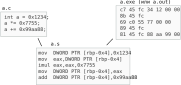
\includegraphics[scale=0.9]{../images/code_to_hex.png}
\end{center}
\subsubsection*{Из кода на C в код ассемблера:}
\begin{itemize}
\item Код на языке \texttt{C} (\texttt{a.c}) переводится в код на языке ассемблера (\texttt{a.s}). Эту операцию можно сделать командой
\begin{verbatim}
gcc -S -masm=intel ./a.c
\end{verbatim}
\item Регистры процессора -- это сверхбыстрая память, которая находится внутри процессора. Её размер очень мал(десятки байт), но процессор может доступиться к ней очень быстро (за 1 такт). В примере выше используются 2 регистра: \texttt{rbp} и \texttt{eax} (\texttt{eax} это часть регистра \texttt{rax}). 
\item Процессор может делать множество различных операций. Например, он может переместить некоторое количество байт из одного места в другое. Такие операции называются \texttt{mov}. Он может прибавить число (\texttt{add}) или умножить на целое (\texttt{imull}) и многое другое. \texttt{DWORD PTR} просто означает, что операция будет работать с 4-мя байтами.
\item В примере выше в регистре \texttt{rbp} содержится некоторый адрес. Квадратные скобочки означают разыменование. Поэтому строка
\begin{verbatim}
mov DWORD PTR [rbp-0x4],0x1234
\end{verbatim}
означает, что нужно положить число \texttt{0x1234} в 4 байта по адресу \texttt{rbp-0x4}
\item 
\begin{verbatim}
mov eax,DWORD PTR [rbp-0x4]
\end{verbatim}
означает, что нужно переместить 4 байта, которые хранятся по адресу \texttt{rbp-0x4} в регистр \texttt{eax}.
\item
\begin{verbatim}
imull eax,eax,0x7755
\end{verbatim}
означает, что нужно умножить содержимое \texttt{eax} на \texttt{0x7755} и сохранить результат в \texttt{eax}.
\item
\begin{verbatim}
mov  DWORD PTR [rbp-0x4],eax
\end{verbatim}
означает, что нужно переместить содержимое \texttt{eax} в память по адресу \texttt{rbp-0x4}.
\item
\begin{verbatim}
add  DWORD PTR [rbp-0x4],0x99aa88
\end{verbatim}
означает, что нужно добавить к числу по адресу \texttt{rbp-0x4} число \texttt{0x99aa88}.
\item В отличии от кода на языке \texttt{C}, код на языке ассемблера различаться на разных процессорах. Код с  вычислительной системы одной архитектуры скорей всего не будет работать на другой.
\end{itemize}
\subsubsection*{Из кода ассемблера в бинарный код (\texttt{.exe}):}
\begin{itemize}
\item Код на языке ассемблера (\texttt{a.s}) переводится в исполняемый файл. Эту операцию можно сделать командой \texttt{gcc a.s}
\item Каждая операция кодируется некоторым числом, называемым кодом операции (opcode).
\item Код операции \texttt{mov} на процессорах архитектуры \texttt{x86-64} может равняться \texttt{с7} или \texttt{8b} или \texttt{89} или некоторым другим  значениям(в зависимости от того куда и откуда мы копируем).
\item Например в строке:
\begin{verbatim}
c7 45 fc 34 12 00 00
\end{verbatim}
\begin{itemize}
\item \texttt{с7} означает, что это операция \texttt{mov} (присвоить число переменной в памяти)
\item \texttt{45} кодирует регистр \texttt{rbp}
\item \texttt{fc} кодирует смещение \texttt{-0x4}
\item \texttt{34 12 00 00} -- это 4-х байтовое число \texttt{0x1234} (порядок байт -- Little Endian)
\end{itemize}

\item
\begin{verbatim}
8b 45 fc
\end{verbatim}
\begin{itemize}
\item \texttt{8b} означает, что это операция \texttt{mov} (записать число, хранящееся в памяти, в \texttt{eax})
\item \texttt{45} кодирует регистр \texttt{rbp}
\item \texttt{fc} кодирует смещение \texttt{-0x4}
\end{itemize}

\item Все коды можно посмотреть тут \href{http://ref.x86asm.net/coder64.html}{ref.x86asm.net/coder64.html}
\item Получается, что в результате компиляции программы код превращается в последовательность байт (инструкций процессора). Эта последовательность байт и хранится в сегменте Текст.
\item А указатель на функцию является просто номером первого байта, с которого начинается функция в этом сегменте.
\item Менять сегмент Текст во время выполнения программы в большинстве современных операционных систем нельзя. 
\end{itemize}



\newpage


\begin{lstlisting}
#include <stdio.h>
#include <stdlib.h>

int array_data[30];

int main() 
{
    int array_stack[30];
    int* array_heap = (int*)malloc(5 * sizeof(int));
    
    printf("%15s %15s %15s\n", "data", "stack", "heap");
    for (int i = 0; i < 30; ++i)
    {
        printf("%15i %15i %15i\n", array_data[i], array_stack[i], array_heap[i]);
    }
    
    free(array_heap);
}
\end{lstlisting}
\end{document}